% !TEX root=../MA119-Main.tex


\paragraph*{Exponential Functions}
	Let $b$ be a positive number other than $1$ (i.e. $b>0$ and $b\neq 1$). The exponential function $f$ of $x$ with the base $b$ is defined as
	\[f(x)=b^x\quad\quad\text{or}\quad\quad y=b^x.\]

	Graphs of exponential functions:
	\begin{multicols}{2}
		\begin{center}
			\begin{tikzpicture}[scale=0.9]
				\begin{axis}[%grid=both,
						unit vector ratio*=1 1,
						ymin=-0.5,ymax=3,xmax=4,xmin=-4, xtick=\empty,ytick=\empty, extra y ticks={1},
						axis lines = middle,xlabel=$x$,ylabel=$y$,
						x label style={anchor=west}, y label style={anchor=south},
						%label style ={at={(ticklabel cs:1.1)}, font={\tiny}}
					]
					% \addplot[thick, samples=100, domain=-3.75:3.75]   {2^x};
					\addplot[thick, samples=100, domain=-3.75:3.75]   {(1/3)^x};
					\node[anchor=east] at (axis cs:-1,2)   {\parbox{2cm}{$f(x)=b^x$\\ $0< b<1$}};
					% \node[anchor=west] at (axis cs:1,2)   {\parbox{2cm}{$f(x)=b^x$\\ $b>1$}};
					\node[circle,fill=black,inner sep=0pt,minimum size=4pt] at (0,1) {};
				\end{axis}
			\end{tikzpicture}
		\end{center}

		\columnbreak

		\begin{center}
			\begin{tikzpicture}[scale=0.9]
				\begin{axis}[%grid=both,
						unit vector ratio*=1 1,
						ymin=-0.5,ymax=3,xmax=4,xmin=-4, xtick=\empty,ytick=\empty, extra y ticks={1},
						axis lines = middle,xlabel=$x$,ylabel=$y$,
						x label style={anchor=west}, y label style={anchor=south},
						%label style ={at={(ticklabel cs:1.1)}, font={\tiny}}
					]
					\addplot[thick, samples=100, domain=-3.75:3.75]   {2^x};
					% \addplot[thick, samples=100, domain=-3.75:3.75]   {(1/2)^x};
					% \node[anchor=east] at (axis cs:-1,2)   {\parbox{2cm}{$f(x)=b^x$\\ $0< b<1$}};
					\node[anchor=west] at (axis cs:1,2)   {\parbox{2cm}{$f(x)=b^x$\\ $b>1$}};
					\node[circle,fill=black,inner sep=0pt,minimum size=4pt] at (0,1) {};
				\end{axis}
			\end{tikzpicture}
		\end{center}
	\end{multicols}

\begin{note}
	The exponential function $f(x)=b^x$ is an one-to-one function: any vertical line or any horizontal line crosses the graph at most once. Equivalently, the equation $b^x=c$ has at most one solution for any real number $c$.
\end{note}
\paragraph*{The Natural Number $e$}
	The natural number $e$ is the number to which the quantity  $\left(1+\dfrac1n\right)^n$ approaches as $n$ takes on increasingly large values.
	Approximately,  $e\approx2.718281827$.

	\paragraph*{Compound Interests}
	After $t$ years, the balance $A$ in an account with a principal $P$ and annual interest rate $r$ is given by the following formulas:

	\begin{enumerate}
		\item For $n$ compounding periods per year: $A=P\left(1+\dfrac{r}{n}\right)^{nt}$.
		\item For compounding continuously: $A=Pe^{rt}$.
	\end{enumerate}

	\begin{example}
		A sum of $\$10,000$ is invested at an annual rate of $8\%$, Find the balance, to the nearest hundredth dollar,  in the account after $5$ years if the interest is compounded \\
		\begin{enumerate*}[label={(\arabic*)~}]
			\item monthly,
			\item quarterly,
			\item semiannually,
			\item continuous.\hfill\null
		\end{enumerate*}
	\end{example}
	\begin{solution}
		\mbox{}\vspace{-0.25em}
		\begin{enumerate}[label={\textbf{\textup{Step \arabic*.}}~}]
			\item Find values of $P$, $r$, $t$ and $n$. In this case,
					$P=10,000$, $r=8\%=0.08$, $t=5$ and $n$ depends compounding.
			\item Plug the values in the formula and calculate.
					\begin{enumerate}[label=\emph{(\arabic*)~}]
						\item ``Monthly'' means $n=12$. Then
							\[A=10000\left(1+\frac{0.08}{12}\right)^{5\cdot 12}\approx 14898.46.\]
						\item ``Quarterly'' means $n=4$. Then
							\[A=10000\left(1+\frac{0.08}{4}\right)^{5\cdot 4}\approx 14859.47.\]
						\item ``semiannually'' means $n=2$. Then
							\[A=10000\left(1+\frac{0.08}{2}\right)^{5\cdot 2}\approx 14802.44.\]
						\item For continuously compounded interest, we have
							\[A=10000e^{0.08\cdot 5}\approx 14918.25.\]
					\end{enumerate}
		\end{enumerate}
	\end{solution}


	\begin{example}
		The population of a country was about 0.78 billion in the year 2015,
		with an annual growth rate of about 0.4\%.
		The predicted population is $P(t)=0.78(1.004)^t$ billions after $t$ years since 2015.
		To the nearest thousandth of a billion, what will the predicted population of the country be in 2030?
	\end{example}

	\begin{solution}
		The population is approximately
		\[
		P(15)=0.78(1.004)^{15}\approx 0.828 \quad \text{billions}.
		\]
	\end{solution}

\newpage

\begin{exercise}
	The value of a car is depreciating according to the formula: $V=25000(3.2)^{-0.05x}$, 
	where $x$ is the age of the car in years. 
	Find the value of the car, to the nearest dollar, when it is five years old.
\end{exercise}


%%%%%%
\vfill
\begin{center} \hfill
	\raisebox{0.4em}{
		\rotatebox{\rotationdegree}{
			\parbox{\textwidth}{
				\begin{enumerate*}[label={\theexer~}]
					\item \$18692 \hfill\null
				\end{enumerate*}
			}
		}
	}
\end{center}



\begin{exercise}
	A sum of \$20,000 is invested at an annual rate of 5.5\%, Find the balance, to the nearest dollar, 
	in the account after 5 years subject to\\
	\begin{enumerate*}[label={(\arabic*)~}]
		\item monthly compounding,
		\item continuously compounding.
		\hfill\null
	\end{enumerate*}
\end{exercise}

%%%%%%
\vfill
\begin{center} \hfill
	\raisebox{0.4em}{
		\rotatebox{\rotationdegree}{
			\parbox{\textwidth}{
				\begin{enumerate*}[label={\theexer~(\arabic*)~}]
					\item \$26314
					\item \$26331
					\hfill\null
				\end{enumerate*}
			}
		}
	}
\end{center}


\newpage

\begin{exercise}
	Sketch the graph of the function and find its range.\\
	\begin{minipage}{\textwidth}
		\begin{minipage}{0.5\textwidth}
			\noindent
			\begin{enumerate*}[label={(\arabic*)~},series=expfungraph]
				\item
				\parbox{0.5\textwidth}{
					$f(x)=3^x$
				}
				\hfill\null
			\end{enumerate*}
			\begin{center}
				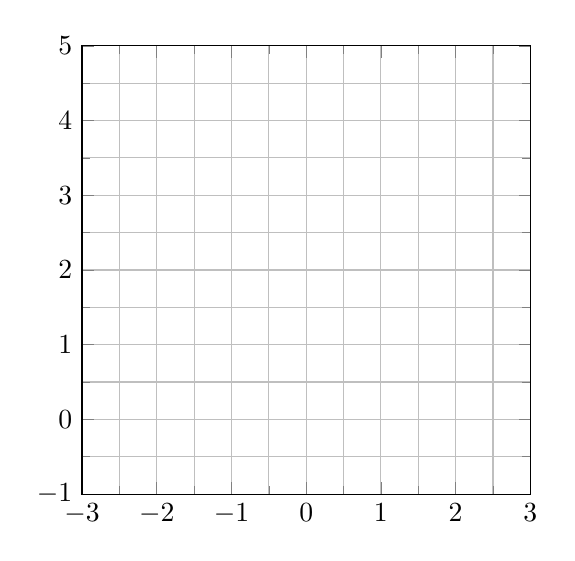
\begin{tikzpicture}[scale=1]
					\begin{axis}[
							grid=both,
							unit vector ratio*=1 1,
							ymin=-1,
							ymax=5,
							xmax=3,
							xmin=-3,
							xtick={-3,-2,...,3},
							ytick={-1,0,...,5},
							minor tick num=1
						]
						%\addplot[thick, samples=100,domain=1:3.82, name path=A, -stealth]   {(x-2)^2+1};
						% \addplot[thick, draw] (1, 2)--(-1.95,1.5);
						% \node[draw,shape=circle, minimum size=1.25mm,inner sep=0pt,outer sep=0pt] at (-2,1.5) {};
					\end{axis}
				\end{tikzpicture}
			\end{center}
		\end{minipage}
		\begin{minipage}{0.5\textwidth}
			\noindent
			\begin{enumerate*}[resume*=expfungraph]
				\item
				\parbox{0.5\textwidth}{
					$f(x)=\left(\frac13\right)^x$
				}
				\hfill\null
			\end{enumerate*}

			\begin{center}
				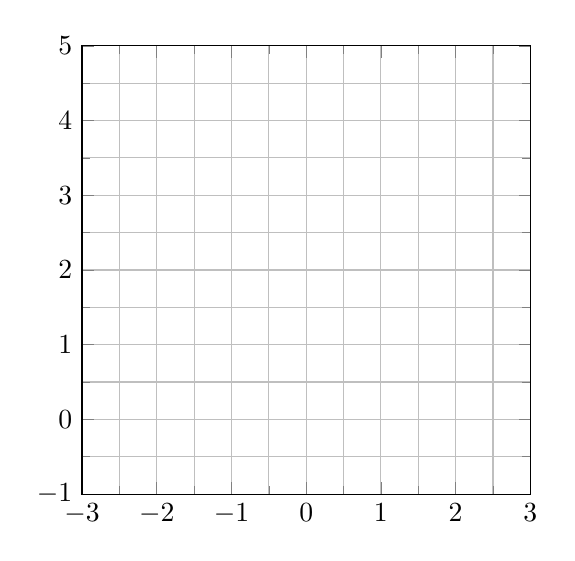
\begin{tikzpicture}[scale=1]
					\begin{axis}[
							grid=both,
							unit vector ratio*=1 1,
							ymin=-1,
							ymax=5,
							xmax=3,
							xmin=-3,
							xtick={-3,-2,...,3},
							ytick={-1,0,...,5},
							minor tick num=1
						]
						%\addplot[thick, samples=100,domain=1:3.82, name path=A, -stealth]   {(x-2)^2+1};
						% \addplot[thick, draw] (1, 2)--(-1.95,1.5);
						% \node[draw,shape=circle, minimum size=1.25mm,inner sep=0pt,outer sep=0pt] at (-2,1.5) {};
					\end{axis}
				\end{tikzpicture}
			\end{center}
		\end{minipage}
	\end{minipage}
\end{exercise}

\vfill

\begin{exercise}Use the given function to compare the values of $f(-1.05)$, $f(0)$ and $f(2.4)$ and determine which value is the largest and which value is the smallest. Explain your answer. \\
	\noindent
	\begin{enumerate*}[label={(\arabic*)~}]
		\item $f(x)=\left(\frac{5}{2}\right)^x$
		\item $f(x)=\left(\frac23\right)^x$
		\hfill\null
	\end{enumerate*}
\end{exercise}

%%%%%%
\vfill
\begin{center} \hfill
	\raisebox{0.4em}{
		\rotatebox{\rotationdegree}{
			\parbox{\textwidth}{
				\begin{enumerate*}[label={\theexer~(\arabic*)~}]
					\item Largest: $f(2.4)$; Smallest: $f(-1.05)$.
					\item Largest: $f(-1.05)$; Smallest: $f(2.4)$.
					\hfill\null
				\end{enumerate*}
			}
		}
	}
\end{center}
